\documentclass[11pt]{article}
\usepackage{../emch574-homework}
\homeworknumber{01}
\studentname{J.C. Vaught}
\duedate{TBD}
\begin{document}
\makehomeworktitle
\begingroup\small\sloppy\tableofcontents\endgroup
\newpage
\subsection*{Assignment}
\noindent\textbullet\quad G signifies students that take this class for Graduate Credit;\par
they must do all the items\par
\noindent\textbullet\quad UG students are not required to do the G work, but they may\par
do it for bonus points\par
\noindent\textbullet\quad Problems solved beyond the minimum requirements will be\par
given bonus points.\par
\noindent\textbullet\quad Challenge problems are optional; they will earn bonus\par
points.\par

\subsection*{NOTES}
\noindent\textbullet\quad Show your work to obtain partial credit if appropriate\par
\noindent\textbullet\quad Always display input data!\par
\noindent\textbullet\quad Partial credit might be given based on work done and\par
MATLAB codes if they are attached; without them, no partial credit can be given.\par
\noindent\textbullet\quad Display numerical results to three significant digits (four if\par
the first digit is 1).\par
\noindent\textbullet\quad Use SI system of measurement\par
https://en.wikipedia.org/wiki/International\_System\_of\_Units\par
\noindent\textbullet\quad Scale units using appropriate prefixes (e.g., nano, micro,\par
milli, kilo, mega, giga...) https://en.wikipedia.org/wiki/Metric\_prefix\par
\noindent\textbullet\quad Problems solved beyond the minimum requirements will be\par
given bonus points.\par
\noindent\textbullet\quad Challenge problems are optional. They may be solved for\par
extra credit\par
\noindent\textbullet\quad Normalized plots are plots with the y-axis scaled between\par
-1 and +1. A plotted variable is normalized by dividing it by its maximum absolute value\par
Notations and abbreviations:\par
\noindent\textbullet\quad BVP = boundary value problem\par
\noindent\textbullet\quad EOM = equation of motion\par
\noindent\textbullet\quad FBD = free body diagram\par
\noindent\textbullet\quad FRF = frequency response function\par
\noindent\textbullet\quad IVP = initial value problem\par
\noindent\textbullet\quad LHS = left hand side\par
\noindent\textbullet\quad NLM = Newton’s law of motion\par
\noindent\textbullet\quad ODE = ordinary differential equation\par
\noindent\textbullet\quad PDE = partial differential equation\par
\noindent\textbullet\quad RHS = right hand side\par
\begin{center}
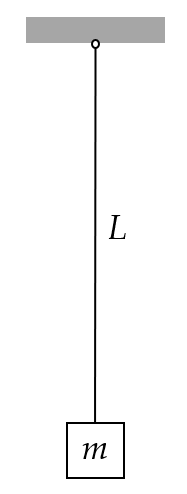
\includegraphics[width=0.72\linewidth,height=0.28\textheight,keepaspectratio]{figures/extracted-000.png}
\end{center}
\section{Pendulum}
\subsection{A.1 ANALYZE PENDULUM}

\begin{center}\small\itshape Figure 1: pendulum of length L and mass m\end{center}

Consider a pendulum of length L and mass m as shown in Figure 1. Do the following:\par
\hangindent=2em\noindent\textbf{(1)} Draw the pendulum displaced by an angle θ from the vertical\par
\hangindent=2em\noindent\textbf{(2)} Draw free-body diagram (FBD)\par
\hangindent=2em\noindent\textbf{(3)} Write Newton’s law of motion (NLM) equation\par
\hangindent=2em\noindent\textbf{(4)} Apply small-angle approximation and deduce the equation of\par
motion (EOM). Clearly state your assumptions.\par
\hangindent=2em\noindent\textbf{(5)} Deduce the governing equation.\par
\hangindent=2em\noindent\textbf{(6)} Assume θ(t)=est and substitute into the governing equation\par
\hangindent=2em\noindent\textbf{(7)} Deduce and solve the characteristic equation\par
\hangindent=2em\noindent\textbf{(8)} How are the roots s1,2? Choose one of the following options:\par
\hangindent=2em\noindent\textbf{(a)} real\par
\hangindent=2em\noindent\textbf{(b)} imaginary\par
\hangindent=2em\noindent\textbf{(c)} complex\par
\hangindent=2em\noindent\textbf{(9)} Define the natural frequency ωn\par
\hangindent=2em\noindent\textbf{(10)} Express the solutions s1 and s2 of the characteristic equation in\par
terms of ωn\par
\hangindent=2em\noindent\textbf{(11)} Write the solution in terms of exponential functions of ωnt\par
\hangindent=2em\noindent\textbf{(12)} Write the solution in terms of trigonometric functions of ωnt\par
\hangindent=2em\noindent\textbf{(13)} write the Hz frequency fn\par
\hangindent=2em\noindent\textbf{(14)} write the period of oscillation τ\par
\hangindent=2em\noindent\textbf{(15)} write the particle motion u(t) in terms of\par
\hangindent=2em\noindent\textbf{(a)} exponential functions\par
\hangindent=2em\noindent\textbf{(b)} trigonometric functions\par
\hangindent=2em\noindent\textbf{(16)} solve the initial value problem (IVP) and find the response u(t)\par
for:\par
\hangindent=2em\noindent\textbf{(i)} initial displacement u0\par
\hangindent=2em\noindent\textbf{(ii)} initial velocity u̇0\par
\hangindent=2em\noindent\textbf{(iii)} simultaneous application of both initial displacement u0\par
and initial velocity u̇0\par
\begin{center}
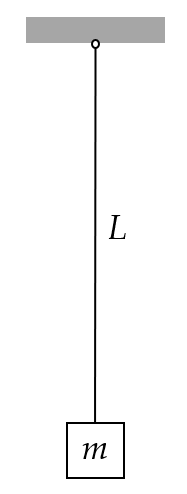
\includegraphics[width=0.72\linewidth,height=0.28\textheight,keepaspectratio]{figures/extracted-005.png}
\end{center}
\subsection{A.2 CALCULATE PENDULUM RESPONSE TO INITIAL}
\subsubsection*{Displacement}

\begin{center}\small\itshape Figure 2: pendulum of length L and mass m\end{center}

Take g=9.81 m/s2 as the generally accepted value of gravitational acceleration. Consider a pendulum of nominal length Lnominal=565mm and mass m=52kg as shown in Figure 2. When manufactured in series production, the pendulum length values are not exact due to manufacturing tolerance. The mm length values for ten pendulum sets are: L = [561.535, 562.691, 563.845, 563.845, 565.0, 565.0, 566.155, 566.155, 567.309, 568.464] mm Do the following:\par
\hangindent=2em\noindent\textbf{(1)} For the ten pendulum sets, calculate\par
\hangindent=2em\noindent\textbf{(a)} rad/sec natural frequency ωn\par
\hangindent=2em\noindent\textbf{(b)} Hz natural frequency fn\par
\hangindent=2em\noindent\textbf{(c)} period of oscillation τ\par
\hangindent=2em\noindent\textbf{(d)} display in table format L, ωn, fn, τ\par
\hangindent=2em\noindent\textbf{(2)} Mean values: calculate and display the mean values of ωn, fn, τ\par
\hangindent=2em\noindent\textbf{(3)} Initial value problem (IVP): assume initial displacement\par
u0=2mm and zero initial velocity. Use the mean values of ωn, fn, τ to do the following:\par
\hangindent=2em\noindent\textbf{(a)} Calculate and display the position of the mass u(t1) after\par
t1=10 sec\par
\hangindent=2em\noindent\textbf{(b)} Calculate and display the duration tNosc of Nosc oscillations\par
and the corresponding position of the mass uNosc for Nosc=10\par
\hangindent=2em\noindent\textbf{(c)} Plot the response of the system for Nosc oscillations and use\par
a datatip on the plot to find the value u(t1) at t1\par
\begin{center}
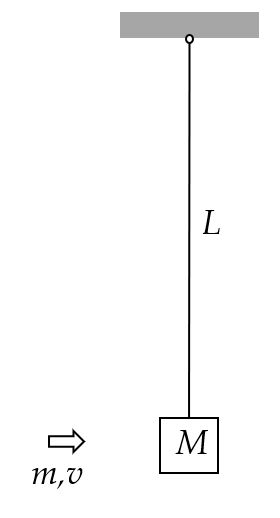
\includegraphics[width=0.72\linewidth,height=0.28\textheight,keepaspectratio]{figures/extracted-008.png}
\end{center}
\subsection{A.3 CALCULATE PENDULUM RESPONSE TO IMPACT}

\begin{center}\small\itshape Figure 3: impact excitation of a pendulum system\end{center}

Take g=9.81 m/s2 as the generally accepted value of gravitational acceleration. Consider a pendulum of nominal length L=565 mm and mass M=52kg as shown in Figure 3. The pendulum is initially at rest hanging vertically. A small projectile of mass m=22 grams and velocity v=945 m/s hits the mass M and remains embedded into it. This impact imparts an initial velocity to the system that starts to oscillate. Do the following:\par
\hangindent=2em\noindent\textbf{(1)} display input data\par
\hangindent=2em\noindent\textbf{(2)} Calculate the rad/sec natural frequency ωn and period of\par
oscillation τ of the pendulum with projectile embedded into it\par
\hangindent=2em\noindent\textbf{(3)} Calculate the initial velocity of the system u̇0 as a result of the\par
interaction between the projectile and the mass.\par
\hangindent=2em\noindent\textbf{(4)} Calculate the response u(t1) after t1=10 sec\par
\hangindent=2em\noindent\textbf{(5)} Plot the response of the system for Nosc=10 oscillations and find\par
on the plot:\par
\hangindent=2em\noindent\textbf{(a)} the largest response\par
\hangindent=2em\noindent\textbf{(b)} the response value calculated at item (4)\par
\hangindent=2em\noindent\textbf{(6)} Discuss your results\par
\begin{center}
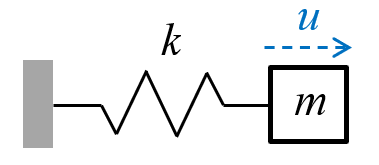
\includegraphics[width=0.72\linewidth,height=0.28\textheight,keepaspectratio]{figures/extracted-013.png}
\end{center}
\section{Spring-Mass-Damper Vibrating Systems}
\subsection{B.1 ANALYZE SPRING-MASS VIBRATING SYSTEM}

\begin{center}\small\itshape Figure 4: spring-mass vibrating system\end{center}

Consider a spring-mass vibrating system as shown in Figure 4. Do the following:\par
\hangindent=2em\noindent\textbf{(1)} Draw free-body diagram (FBD)\par
\hangindent=2em\noindent\textbf{(2)} Write NLM equation\par
\hangindent=2em\noindent\textbf{(3)} Deduce the equation of motion (EOM)\par
\hangindent=2em\noindent\textbf{(4)} Deduce the governing equation. Clearly state your assumptions.\par
\hangindent=2em\noindent\textbf{(5)} Assume u(t)=est and substitute into the governing equation\par
\hangindent=2em\noindent\textbf{(6)} Deduce the characteristic equation\par
\hangindent=2em\noindent\textbf{(7)} Define the natural frequency ωn in terms of m,k\par
\hangindent=2em\noindent\textbf{(8)} Solve the characteristic equation and find s1,2 in terms of ωn\par
\hangindent=2em\noindent\textbf{(9)} Answer the following question: How are the roots s1,2? Choose\par
one of the following options:\par
\hangindent=2em\noindent\textbf{(a)} real\par
\hangindent=2em\noindent\textbf{(b)} imaginary\par
\hangindent=2em\noindent\textbf{(c)} complex\par
\hangindent=2em\noindent\textbf{(10)} Write the solution in terms of exponential functions\par
\hangindent=2em\noindent\textbf{(11)} Write the solution in terms of trigonometric functions\par
\hangindent=2em\noindent\textbf{(12)} Solve the initial value problem (IVP) and find the response u(t)\par
for:\par
\hangindent=2em\noindent\textbf{(i)} initial displacement u0\par
\hangindent=2em\noindent\textbf{(ii)} initial velocity u̇0\par
\hangindent=2em\noindent\textbf{(iii)} simultaneous application of both initial displacement u0\par
and initial velocity u̇0\par
\begin{center}
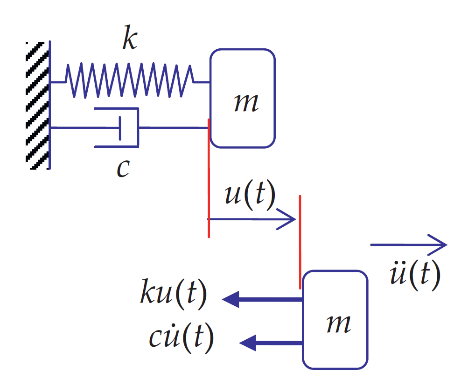
\includegraphics[width=0.72\linewidth,height=0.28\textheight,keepaspectratio]{figures/extracted-014.png}
\end{center}
\subsection{B.2 ANALYZE SPRING-MASS-DAMPER VIBRATING SYSTEM}
Consider the 1-dof damped system consisting of a spring, k, mass, m, and viscous damper, c, as presented in Figure 5. Assume the mass m is displaced from the equilibrium position by a time-dependent displacement u(t).\par

\begin{center}\small\itshape Figure 5 mass-spring-damper vibrating system\end{center}

Do the following:\par
\hangindent=2em\noindent\textbf{(1)} State your assumptions in performing this analysis\par
\hangindent=2em\noindent\textbf{(2)} Draw free-body diagram (FBD) and deduce the sum of forces\par
in the x direction.\par
\hangindent=2em\noindent\textbf{(3)} Write NLM equation\par
\hangindent=2em\noindent\textbf{(4)} Deduce the equation of motion (EOM) as an ODE in terms of\par
m, c, k\par
\hangindent=2em\noindent\textbf{(5)} Assume u(t)=est and substitute into EOM\par
\hangindent=2em\noindent\textbf{(6)} Deduce the characteristic equation\par
\hangindent=2em\noindent\textbf{(7)} Find the roots s1,2 of the characteristic equation\par
\hangindent=2em\noindent\textbf{(8)} Define critical damping ccr in terms of m and k\par
\hangindent=2em\noindent\textbf{(9)} Define damping ratio ζ\par
\hangindent=2em\noindent\textbf{(10)} Discuss the values of ζ for the three damping cases:\par
\hangindent=2em\noindent\textbf{(a)} underdamped\par
\hangindent=2em\noindent\textbf{(b)} critically damped\par
\hangindent=2em\noindent\textbf{(c)} overdamped\par
\hangindent=2em\noindent\textbf{(11)} Express the physical damping c in terms of damping ratio ζ,\par
mass m, stiffness k\par
\hangindent=2em\noindent\textbf{(12)} Define the natural frequency ωn in terms of m,k\par
\hangindent=2em\noindent\textbf{(13)} Express in terms of ωn, ζ the s1,2 roots found at (7)\par
\hangindent=2em\noindent\textbf{(14)} Assume underdamped system and express the s1,2 roots of (13)\par
as complex numbers in terms of ωn and ζ\par
\hangindent=2em\noindent\textbf{(15)} Define the damped frequency ωd\par
\hangindent=2em\noindent\textbf{(16)} Substitute (15) into (14) and express the roots s1 and s2 in terms\par
of ωn, ωd, ζ\par
\hangindent=2em\noindent\textbf{(17)} Assume underdamped conditions and state the inequality that\par
ζ should satisfy\par
\hangindent=2em\noindent\textbf{(18)} Write the general solution of the ODE deduced at (4) in terms\par
of some constants C1, C2 multiplying exponential functions of s1 , s2\par
\hangindent=2em\noindent\textbf{(19)} Use (16) to write the solution (18) in terms of exponential\par
functions of ωn, ωd, ζ\par
\hangindent=2em\noindent\textbf{(20)} Rewrite the solution (19) in terms of an exponential decay\par
function multiplying the sum of two complex exponentials\par
\hangindent=2em\noindent\textbf{(21)} Rewrite the solution (20) in terms of an exponential decay\par
function multiplying a trigonometric function and some constants C and φ to be determined from the initial conditions.\par
\hangindent=2em\noindent\textbf{(22)} Sketch the functions discussed at (21)\par
\hangindent=2em\noindent\textbf{(23)} Solve the initial value problem (IVP) for ζ<1 and find the\par
response u(t) for initial displacement u0 with zero initial velocity\par
\hangindent=2em\noindent\textbf{(24)} Solve the initial value problem (IVP) and find the response\par
u(t) for simultaneous application of initial displacement u0 and initial velocity u̇0\par
\begin{center}
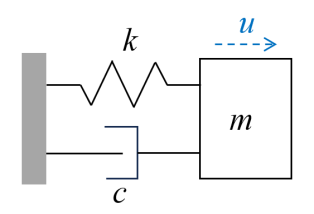
\includegraphics[width=0.72\linewidth,height=0.28\textheight,keepaspectratio]{figures/extracted-017.png}
\end{center}
\subsection{B.3 CALCULATE SPRING-MASS-DAMPER RESPONSE TO INITIAL}
\subsubsection*{Displacement}

\begin{center}\small\itshape Figure 6: spring-mass-damper vibrating system\end{center}

Consider a spring-mass vibrating system with m=12 kg, k=655 N/m, c=19 N/(m/s) as shown in Figure 6. The vibrating system is given an initial displacement u0=3.5 mm with zero initial velocity. Do the following:\par
\hangindent=2em\noindent\textbf{(1)} Display input data\par
\hangindent=2em\noindent\textbf{(2)} Calculate the natural frequency in rad/sec ωn and in Hz fn\par
\hangindent=2em\noindent\textbf{(3)} Calculate the critical damping ccr\par
\hangindent=2em\noindent\textbf{(4)} Calculate the damping ratio ζ\par
\hangindent=2em\noindent\textbf{(5)} Calculate the damped frequency in rad/sec ωd and in Hz fd\par
\hangindent=2em\noindent\textbf{(6)} Calculate the damped period of oscillation τd\par
\hangindent=2em\noindent\textbf{(7)} Calculate the characteristic-equation roots s1, s2 and the\par
constants C1, C2\par
\hangindent=2em\noindent\textbf{(8)} Calculate the constants A, B and then the constants C, φ\par
\hangindent=2em\noindent\textbf{(9)} Calculate the duration t1 of one oscillation and the\par
corresponding position u1=u(t1)\par
\hangindent=2em\noindent\textbf{(10)} Calculate the value u0.02 representing 2\% of the initial\par
displacement\par
\hangindent=2em\noindent\textbf{(11)} Plot the response of the system for Nosc=10 oscillations and use\par
datatips on the plot to find the following:\par
\hangindent=2em\noindent\textbf{(a)} the largest response\par
\hangindent=2em\noindent\textbf{(b)} the response value calculated at item (9)\par
\hangindent=2em\noindent\textbf{(c)} the time when the response magnitude has decreased\par
permanently below u0.02 calculated at item (10)\par
\hangindent=2em\noindent\textbf{(12)} Discuss your results\par
\begin{center}
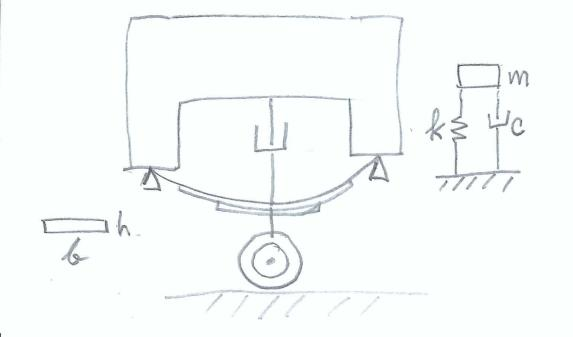
\includegraphics[width=0.72\linewidth,height=0.28\textheight,keepaspectratio]{figures/extracted-020.png}
\end{center}
\subsection{B.4 CALCULATE TRUCK SUSPENSION RESPONSE}
Consider a pickup truck wheel suspension consisting of a leaf spring and an oil damper. The truck and its suspension can be modeled, in first approximation, as a k-m-c spring-mass-damper system as shown in Figure 7.\par

\begin{center}\small\itshape Figure 7 Truck suspension consisting of a leaf spring and an oil damper\end{center}

The leaf spring can be approximated by a uniform beam of length L=830 mm and cross-section dimensions h=3mm, b=65 mm made of steel with E=200GPa. The truck mass apportioned to the wheel can be estimated as m=457kg. Assume initial displacement u0=125mm and zero initial velocity u̇0 = 0 . Do the following:\par
\hangindent=2em\noindent\textbf{(1)} Display input data\par
\hangindent=2em\noindent\textbf{(2)} Calculate the second moment of area I of the beam cross-\par
section\par
\hangindent=2em\noindent\textbf{(3)} Calculate the flexural stiffness EI of the beam\par
\hangindent=2em\noindent\textbf{(4)} Calculate the spring constant k of the system\par
\hangindent=2em\noindent\textbf{(5)} Calculate the natural frequency in rad/sec ωn and in Hz fn\par
\hangindent=2em\noindent\textbf{(6)} Calculate the critical damping ccr\par
\hangindent=2em\noindent\textbf{(7)} Assume 25\% damping ratio, i.e., ζ=0.25, and calculate the\par
physical damping c. Print ζ and c\par
\hangindent=2em\noindent\textbf{(8)} Calculate the damped frequency in rad/sec ωd and in Hz fd\par
\hangindent=2em\noindent\textbf{(9)} Calculate the damped period of oscillation τd\par
\hangindent=2em\noindent\textbf{(10)} Calculate the characteristic-equation roots s1, s2 and the\par
constants C1, C2\par
\hangindent=2em\noindent\textbf{(11)} Calculate the constants A, B and then the constants C, φ\par
\hangindent=2em\noindent\textbf{(12)} Calculate the duration t1 of one oscillation and the\par
corresponding position u1=u(t1)\par
\hangindent=2em\noindent\textbf{(13)} Calculate the value u0.02 representing 2\% of the initial\par
displacement\par
\hangindent=2em\noindent\textbf{(14)} Plot the response of the system for Nosc=10 oscillations and use\par
datatips on the plot to find the following:\par
\hangindent=2em\noindent\textbf{(a)} the largest response\par
\hangindent=2em\noindent\textbf{(b)} the response value calculated at item (11)\par
\hangindent=2em\noindent\textbf{(a)} the time when the response magnitude has decreased\par
permanently below u0.02 calculated at item (13)\par
\hangindent=2em\noindent\textbf{(15)} Discuss your results\par
\hangindent=2em\noindent\textbf{(16)} Graduate work: assume the damper is worn out such that ζ is\par
reduced to ζ=10\%.\par
\hangindent=2em\noindent\textbf{(a)} Repeat the calculation of items (6) through (12)\par
\hangindent=2em\noindent\textbf{(b)} Compare and discuss the two results\par
\subsection{B.5 OVERDAMPED SPRING-MASS-DAMPER SYSTEMS}
Consider a spring-mass-damper system with natural frequency fn=6.25 Hz and various values of the damping ratio ζ. The system is given an initial displacement u0 = 13 mm with zero initial velocity. Do the following:\par
\hangindent=2em\noindent\textbf{(1)} display input data\par
\hangindent=2em\noindent\textbf{(2)} calculate the rad/s frequency ωn\par
\hangindent=2em\noindent\textbf{(3)} Assume overdamped conditions ζ > 1 and develop the solution\par
as follows:\par
\hangindent=2em\noindent\textbf{(a)} write the expressions of the roots s1, s2 in terms of ωn and ζ\par
\hangindent=2em\noindent\textbf{(b)} write the solution u(t) in terms of s1, s2 and constants C1, C2\par
\hangindent=2em\noindent\textbf{(c)} write the expression of the constants C1, C2 in terms of initial\par
displacement u0 and initial velocity u̇0\par
\hangindent=2em\noindent\textbf{(d)} take ζ=2.3 and calculate the numerical values of s1, s2 and\par
\subsubsection*{C1, C2}
\hangindent=2em\noindent\textbf{(e)} plot the response u(t) for t=0,...,3 seconds\par
\hangindent=2em\noindent\textbf{(4)} Assume critically damped conditions ζ =1 and do the following:\par
\hangindent=2em\noindent\textbf{(a)} write the expressions of the two partial solutions u1(t), u2(t)\par
in terms of ωn\par
\hangindent=2em\noindent\textbf{(b)} write the expression of the complete solution in terms of ωn\par
and C1, C2\par
\hangindent=2em\noindent\textbf{(c)} write the expressions of the constants C1, C2 in terms of\par
initial displacement u0 and initial velocity u̇0\par
\hangindent=2em\noindent\textbf{(d)} calculate the numerical values of C1, C2\par
\hangindent=2em\noindent\textbf{(e)} plot the response u(t) for t=0,...,3 seconds\par
\hangindent=2em\noindent\textbf{(5)} Graduate Work: derive the ODE for ζ =1 and verify that the\par
two solutions u1(t) and u2(t) from (4)(a) satisfy the ODE\par
\hangindent=2em\noindent\textbf{(6)} Graduate Work: some race-car manufacturers design for\par
critical damping whereas others use overdamped design. Discuss the pros and cons of the two options\par
\begin{center}
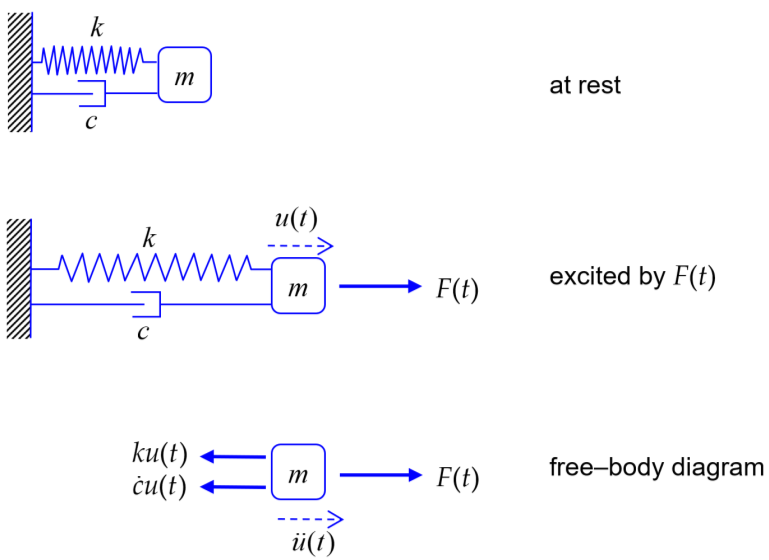
\includegraphics[width=0.72\linewidth,height=0.28\textheight,keepaspectratio]{figures/extracted-025.png}
\end{center}
\subsection{B.6 ANALYZE SPRING-MASS-DAMPER FORCED VIBRATION}
Consider a mass-spring-damper vibrating system excited by a time- dependent force F(t) as shown in Figure 8.\par

\begin{center}\small\itshape Figure 8 spring-mass-damper system excited by force F(t)\end{center}

Do the following:\par
\hangindent=2em\noindent\textbf{(1)} State your assumptions in performing this analysis\par
\hangindent=2em\noindent\textbf{(2)} Draw free-body diagram (FBD) and deduce the sum of forces\par
in the x direction.\par
\hangindent=2em\noindent\textbf{(3)} Write NLM equation\par
\hangindent=2em\noindent\textbf{(4)} Deduce the equation of motion (EOM) as an ODE in terms of\par
m, c, k, F(t) ˆ iωt , substitute in (4) and\par
\hangindent=2em\noindent\textbf{(5)} Assume harmonic excitation F(t ) = Fe\par
divide by m\par
\hangindent=2em\noindent\textbf{(6)} Define the normalized excitation amplitude fˆ = Fˆ m and\par
recall the definitions of ωn and ζ to obtain a nonhomogeneous linear ODE in ωn, ζ, f̂\par
\hangindent=2em\noindent\textbf{(7)} Write the general solution u(t) as a sum of a complementary\par
solution uc(t) and a particular solution up(t)\par
\hangindent=2em\noindent\textbf{(8)} Write the general form of the complementary solution uc(t)\par
\hangindent=2em\noindent\textbf{(9)} Find the particular solution up(t)\par
\hangindent=2em\noindent\textbf{(10)} Use (8), (9) to write the complete solution u(t); discuss the\par
meaning of transient response and steady-state response.\par
\hangindent=2em\noindent\textbf{(11)} Find an expression for the steady-state response amplitude uˆ ss\par

in terms of ωn, ζ, f̂ , ω\par
\hangindent=2em\noindent\textbf{(12)} Develop the expression for the frequency response function\par
FRF(ω) in terms of ωn, ζ, ω\par
\hangindent=2em\noindent\textbf{(13)} Discuss the variation with frequency of FRF magnitude and\par
phase\par
\hangindent=2em\noindent\textbf{(14)} Give the definition of the magnification factor M(ω)\par
\hangindent=2em\noindent\textbf{(15)} Give the expression for the magnification factor M(ω) in terms\par
of ωn and ζ\par
\hangindent=2em\noindent\textbf{(16)} Give the definition of the resonance frequency ωr\par
\hangindent=2em\noindent\textbf{(17)} Give the expression for the resonance frequency ωr in terms of\par
ωn and ζ\par
\hangindent=2em\noindent\textbf{(18)} Give the expression of the peak magnification Mr\par
\hangindent=2em\noindent\textbf{(19)} Give the expression of the of the FRF phase φ(p) where\par
p=ω/ωn\par
\hangindent=2em\noindent\textbf{(20)} Give the definition of phase resonance and deduce the FRF\par
expression at phase resonance\par
\hangindent=2em\noindent\textbf{(21)} Calculate the magnification factor at phase resonance\par
\hangindent=2em\noindent\textbf{(22)} Calculate the magnitude of the physical response at phase\par
resonance\par
\hangindent=2em\noindent\textbf{(23)} Discuss the difference between true resonance and phase\par
resonance\par
\hangindent=2em\noindent\textbf{(24)} Write and compare the expressions for the resonance\par
frequency ωr and damped frequency ωd\par
\hangindent=2em\noindent\textbf{(25)} Establish a formula to calculate the RPM corresponding to a\par
rad/sec frequency ω\par
\begin{center}
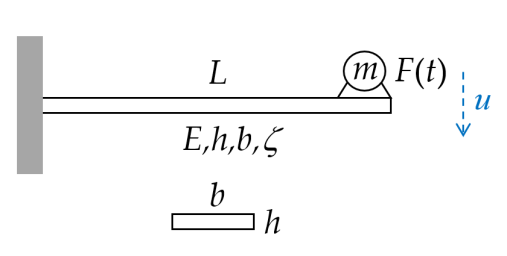
\includegraphics[width=0.72\linewidth,height=0.28\textheight,keepaspectratio]{figures/extracted-026.png}
\end{center}
\subsection{B.7 CALCULATE FLEX-BEAM RESPONSE TO SLIGHTLY}
\subsubsection*{Unbalanced Electric Motor Excitation}

\begin{center}\small\itshape Figure 9 damped cantilever beam excited by force F(t) from slightly\end{center}
unbalanced electric motor\par

Consider a cantilever beam of length L=568 mm, elastic modulus E=200 GPa, cross-section properties h=3 mm, b=37 mm and damping ratio ζ=14\%. (The damping is achieved through a proprietary damping treatment applied on the beam surface.) An electric motor of mass m=0.52kg operating at 1,500 RPM is attached at the beam tip as shown in Figure 9. The electric motor is slightly ˆ iωt with unbalanced producing a slight vibratory excitation F(t ) = Fe F̂ = 12 mN. The excitation frequency ω depends on the electric motor RPM. Do the following:\par
\hangindent=2em\noindent\textbf{(1)} Display input data\par
\hangindent=2em\noindent\textbf{(2)} Calculate\par
\hangindent=2em\noindent\textbf{(a)} cross-section second moment of area I, flexural stiffness EI,\par
and spring constant k\par
\hangindent=2em\noindent\textbf{(b)} natural frequency ωn rad/s, critical damping ccr, physical\par
damping c\par
\hangindent=2em\noindent\textbf{(c)} quasi-static deflection uqst corresponding to ωn->0\par
\hangindent=2em\noindent\textbf{(3)} Calculate the values of\par
\hangindent=2em\noindent\textbf{(a)} resonant frequency ωr and damped frequency ωd\par
\hangindent=2em\noindent\textbf{(b)} peak magnification Mr\par
\hangindent=2em\noindent\textbf{(c)} magnification at phase resonance M90\par
\hangindent=2em\noindent\textbf{(d)} physical response û90 at phase resonance and its magnitude\par
û90\par
\hangindent=2em\noindent\textbf{(e)} calculate the Hz frequencies fr, fn and the corresponding\par
RPM values\par
\hangindent=2em\noindent\textbf{(4)} assume excitation at phase resonance:\par
\hangindent=2em\noindent\textbf{(a)} calculate the excitation frequency ω in rad/s and f in Hz\par
\hangindent=2em\noindent\textbf{(b)} calculate period of oscillation τ\par
\hangindent=2em\noindent\textbf{(c)} Plot the time response for Nosc=10 oscillations. Hint: plot the\par
real part of the complex displacement u(t)\par
\hangindent=2em\noindent\textbf{(5)} Graduate work:\par
\hangindent=2em\noindent\textbf{(a)} calculate and display the operational frequency f0 in Hz and\par
the corresponding ω0 in rad/sec. Plot the magnitude and phase of the frequency response function FRF vs. excitation f in Hz from quasi-static to f0 with Nf=5000 points\par
\hangindent=2em\noindent\textbf{(b)} calculate and display the FRF magnitude at phase-resonance\par
RPM, at double the phase resonance RPM, and at operational RPM. Display the corresponding Hz frequencies. Put the corresponding data tips on the magnitude plot\par
\hangindent=2em\noindent\textbf{(c)} calculate the vibration magnitude |u0| when the electric\par
motor runs at its operational RPM\par
\hangindent=2em\noindent\textbf{(d)} comment on what vibration would be observed as the motor\par
is switched on and accelerates to reach its operational RPM\par
\begin{center}
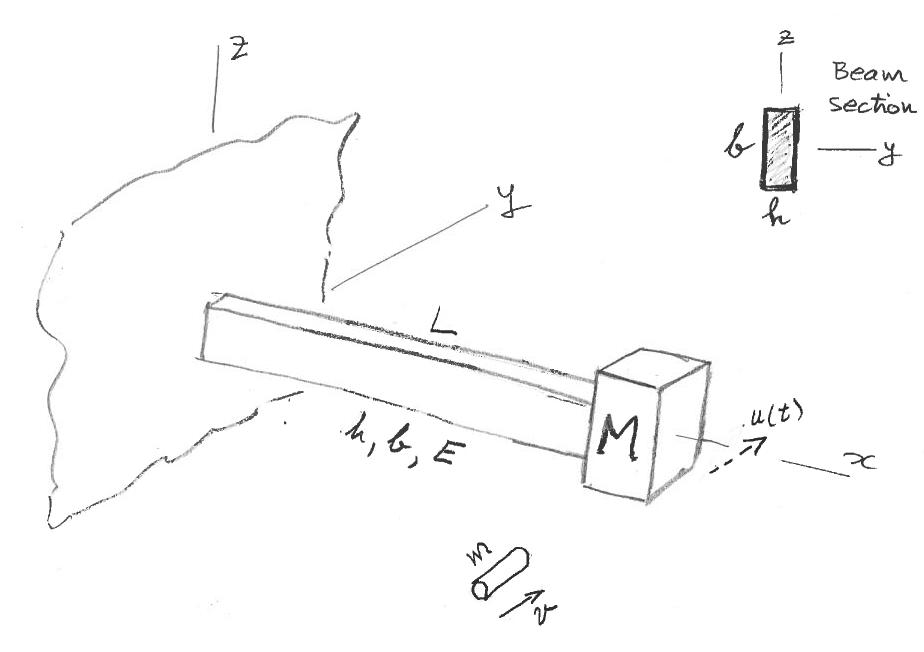
\includegraphics[width=0.72\linewidth,height=0.28\textheight,keepaspectratio]{figures/extracted-029.png}
\end{center}
\subsection{B.8 GRADUATE WORK: CALCULATE}
\subsubsection*{Horizontal Flex-Beam Response To Impact}

\begin{center}\small\itshape Figure 10: impact excitation of a horizontal flex-beam vibration system\end{center}

Consider a cantilever beam of length L=568 mm with a mass M=53kg attached at its tip as shown in Figure 10. The beam material is steel with E=200 GPa. The beam cross-section dimensions are h=3 mm, b=37 mm. The beam is initially at rest. A small projectile of mass m=18 grams and velocity v=935 m/s hits the mass and remains embedded in it. This impact imparts an initial velocity to the system that starts to oscillate with motion u(t) contained in the horizontal plane. Do the following:\par
\hangindent=2em\noindent\textbf{(1)} Display input data\par
\hangindent=2em\noindent\textbf{(2)} Calculate the second moment of area I for flexing consistent\par
with the direction of motion u(t)\par
\hangindent=2em\noindent\textbf{(3)} Calculate the cross-sectional stiffness EI of the beam\par
\hangindent=2em\noindent\textbf{(4)} Calculate the flex-beam spring constant k\par
\hangindent=2em\noindent\textbf{(5)} Calculate the initial velocity of the system u̇0 as a result of the\par
interaction between the projectile and the mass\par
\hangindent=2em\noindent\textbf{(6)} Calculate the rad/sec natural frequency ωn and period of\par
oscillation τ\par
\hangindent=2em\noindent\textbf{(7)} Calculate the position of the mass u(t1) after t1=10 sec\par
\hangindent=2em\noindent\textbf{(8)} Plot the response of the system for Nosc=10 oscillations and find\par
on the plot:\par
\hangindent=2em\noindent\textbf{(a)} the largest response\par
\hangindent=2em\noindent\textbf{(b)} the response calculated at item (7)\par
\hangindent=2em\noindent\textbf{(9)} Discuss your results\par
\begin{center}
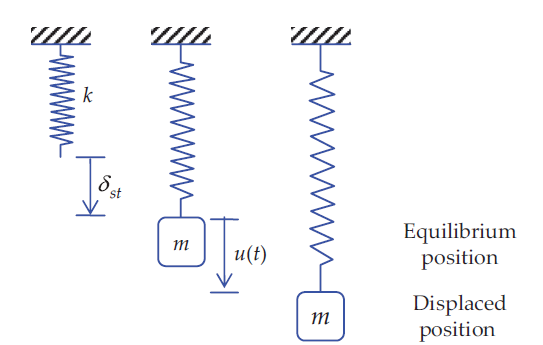
\includegraphics[width=0.72\linewidth,height=0.28\textheight,keepaspectratio]{figures/extracted-030.png}
\end{center}
\section{Extra Credit Challenge Problems}
Challenge problems are optional.\par
\subsection{C.1 ANALYZE VERTICAL SPRING-MASS VIBRATION SYSTEM}

\begin{center}\small\itshape Figure 11 vertical spring-mass vibration system\end{center}

Consider a vertical spring-mass vibration system consisting of a particle of mass m hanging on an elastic spring of stiffness k as shown in Figure 11. Do the following:\par
\hangindent=2em\noindent\textbf{(1)} Assume static equilibrium\par
\hangindent=2em\noindent\textbf{(a)} Calculate the weight W acting on the mass m\par
\hangindent=2em\noindent\textbf{(b)} Draw free-body diagram (FBD)\par
\hangindent=2em\noindent\textbf{(c)} Write equilibrium equation\par
\hangindent=2em\noindent\textbf{(d)} Solve for the static displacement δst\par
\hangindent=2em\noindent\textbf{(2)} Assume vibration with time-varying vertical displacement u(t)\par
\hangindent=2em\noindent\textbf{(a)} Draw free-body diagram (FBD)\par
\hangindent=2em\noindent\textbf{(b)} Deduce equation of motion (EOM)\par
\hangindent=2em\noindent\textbf{(c)} Compare the EOM deduced here with the EOM derived for\par
horizontal spring-mass vibration system of Problem B.1\par
\hangindent=2em\noindent\textbf{(3)} Graduate Work: comment on how the EOM would change in\par
the presence of an arbitrary force field acting at an angle θ wrt vertical axis.\par
\begin{center}
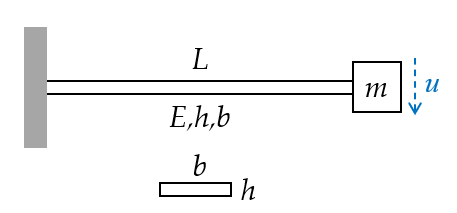
\includegraphics[width=0.72\linewidth,height=0.28\textheight,keepaspectratio]{figures/extracted-031.png}
\end{center}
\subsection{C.2 ANALYZE VERTICAL FLEX-BEAM VIBRATION}

\begin{center}\small\itshape Figure 12: vertical flex-beam vibrating system\end{center}

Consider a cantilever beam of length L with a mass m attached at its tip as shown in Figure 12. The beam cross-section properties are E, h, b. Do the following:\par
\hangindent=2em\noindent\textbf{(1)} Calculate the cross-sectional stiffness EI of the beam for vertical\par
flexural deformation\par
\hangindent=2em\noindent\textbf{(2)} Calculate the spring constant k of the system\par
\hangindent=2em\noindent\textbf{(3)} Assume static equilibrium:\par
\hangindent=2em\noindent\textbf{(a)} Calculate the weight W acting on the mass m\par
\hangindent=2em\noindent\textbf{(b)} Draw free-body diagram (FBD)\par
\hangindent=2em\noindent\textbf{(c)} Write equilibrium equation\par
\hangindent=2em\noindent\textbf{(d)} Solve for the static displacement δst\par
\hangindent=2em\noindent\textbf{(4)} Assume vibration with time-varying vertical displacement u(t)\par
measured from the static equilibrium position:\par
\hangindent=2em\noindent\textbf{(a)} Draw free-body diagram (FBD)\par
\hangindent=2em\noindent\textbf{(b)} Deduce equation of motion (EOM)\par
\hangindent=2em\noindent\textbf{(c)} Compare the EOM deduced here with the EOM derived for\par
horizontal flex-beam vibration system of Problem C.4\par
\hangindent=2em\noindent\textbf{(5)} Graduate Work: comment on how the EOM would change in\par
the presence of an arbitrary force field acting at an angle θ wrt vertical axis.\par
\begin{center}
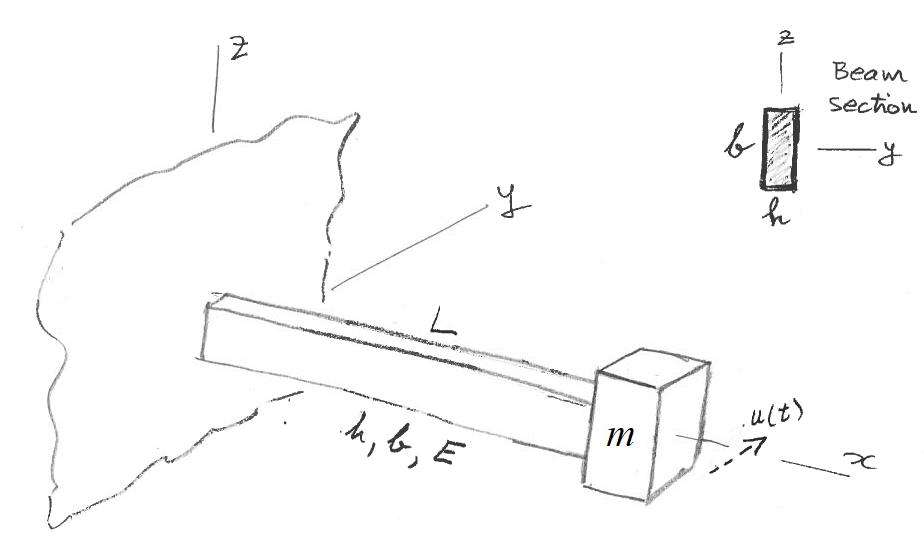
\includegraphics[width=0.72\linewidth,height=0.28\textheight,keepaspectratio]{figures/extracted-034.png}
\end{center}
\subsection{C.3 ANALYZE HORIZONTAL FLEX-BEAM VIBRATION}

\begin{center}\small\itshape Figure 13: horizontal flex-beam vibrating system\end{center}

Consider a cantilever beam of length L with a mass m attached at its tip as shown in Figure 13. The beam cross-section properties are E, h, b. Do the following:\par
\hangindent=2em\noindent\textbf{(1)} Assume vibration with horizontal time-varying displacement\par
u(t) as shown in Figure 13\par
\hangindent=2em\noindent\textbf{(2)} Calculate the cross-sectional stiffness EI of the beam for flexural\par
deformation consistent with u(t)\par
\hangindent=2em\noindent\textbf{(3)} Calculate the flex-beam spring constant k\par
\hangindent=2em\noindent\textbf{(4)} Draw free-body diagram (FBD) including all the forces acting\par
on the mass m\par
\hangindent=2em\noindent\textbf{(5)} Deduce equation of motion (EOM)\par
\hangindent=2em\noindent\textbf{(6)} Compare the EOM deduced here with the EOM derived in\par
Problem B.1\par
\hangindent=2em\noindent\textbf{(7)} Solve the initial value problem (IVP) and find the response for\par
simultaneous application of both initial displacement u0 and initial velocity u̇0\par
\begin{center}
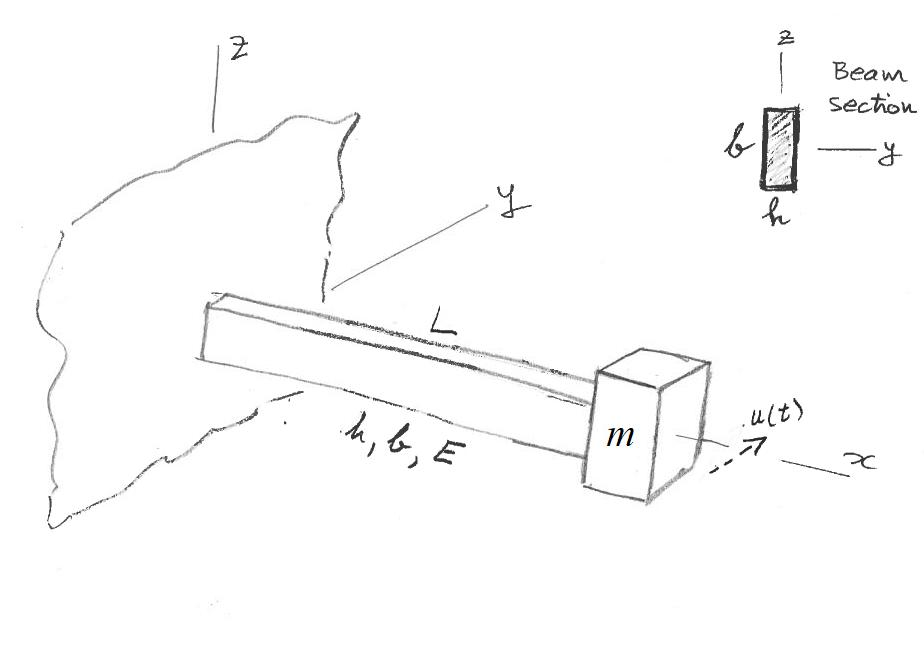
\includegraphics[width=0.72\linewidth,height=0.28\textheight,keepaspectratio]{figures/extracted-035.png}
\end{center}
\subsection{C.4 CALCULATE HORIZONTAL FLEX-BEAM RESPONSE TO}
\subsubsection*{Initial Displacement}

\begin{center}\small\itshape Figure 14: flex-beam vibrating system\end{center}

Consider a cantilever beam of length L=568 mm with a mass m=5.35kg attached at its tip as shown in Figure 14. The beam material is steel with E=200 GPa. The beam cross-section dimensions are h=3 mm, b=37 mm. The tip mass is given an initial displacement u0=5.4mm with zero initial velocity. Do the following:\par
\hangindent=2em\noindent\textbf{(1)} Display input data\par
\hangindent=2em\noindent\textbf{(2)} Calculate the second moment of area I for flexing consistent\par
with the direction of motion u(t)\par
\hangindent=2em\noindent\textbf{(3)} Calculate the cross-sectional stiffness EI of the beam\par
\hangindent=2em\noindent\textbf{(4)} Calculate the spring constant k of the system\par
\hangindent=2em\noindent\textbf{(5)} Calculate the natural frequency in rad/sec ωn\par
\hangindent=2em\noindent\textbf{(6)} Calculate the natural frequency in Hz fn\par
\hangindent=2em\noindent\textbf{(7)} Calculate the period of oscillation in sec τ\par
\hangindent=2em\noindent\textbf{(8)} Calculate the position of the mass u(t1) after t1=10 sec\par
\hangindent=2em\noindent\textbf{(9)} Plot the response of the system for Nosc=25 oscillations and use\par
a data tip on the plot to find the value u(t1) at t1 on the plot\par
\hangindent=2em\noindent\textbf{(10)} Discuss your results\par
\begin{center}
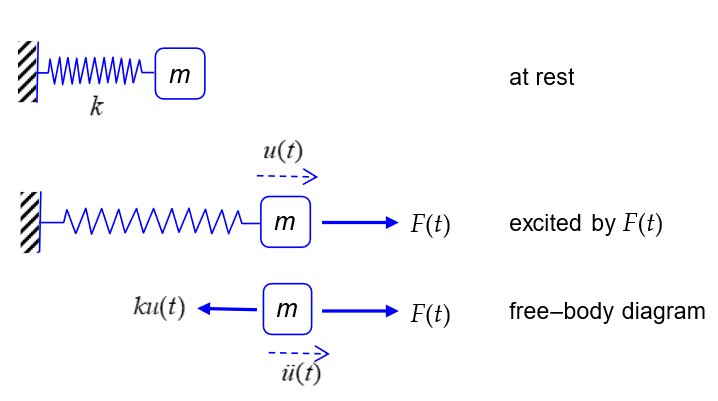
\includegraphics[width=0.72\linewidth,height=0.28\textheight,keepaspectratio]{figures/extracted-036.png}
\end{center}
\subsection{C.5 ANALYZE SPRING-MASS FORCED VIBRATION}
Consider a spring-mass vibrating system excited by a time- dependent force F(t) as shown in Figure 15.\par

\begin{center}\small\itshape Figure 15 spring-mass system excited by force F(t)\end{center}

General analysis of spring-mass forced vibration Do the following:\par
\hangindent=2em\noindent\textbf{(1)} State your assumptions in performing this analysis\par
\hangindent=2em\noindent\textbf{(2)} Draw free-body diagram (FBD) and deduce the sum of forces\par
in the x direction.\par
\hangindent=2em\noindent\textbf{(3)} Write NLM equation\par
\hangindent=2em\noindent\textbf{(4)} Deduce the equation of motion (EOM) and express it as a\par
nonhomogeneous ODE in terms of m, c, k, F(t)\par
\hangindent=2em\noindent\textbf{(5)} Write the ODE general solution as the superposition of a\par
complementary solution uc(t) and a particular solution up(t)\par
\hangindent=2em\noindent\textbf{(6)} Recall the complementary solution uc(t) as the solution of the\par
homogeneous equation studied in HW01 and write it in terms of trigonometric functions multiplied by constants A and B.\par
Analysis of spring-mass response to suddenly applied load\par
\hangindent=2em\noindent\textbf{(7)} Assume the loading F(t) is a suddenly applied load of\par
magnitude F0\par
\hangindent=2em\noindent\textbf{(8)} Find the particular solution for this case of a suddenly applied\par
load\par
\hangindent=2em\noindent\textbf{(9)} Write the complete solution as the sum of uc(t) from (6) and\par
up(t) from (8)\par
\hangindent=2em\noindent\textbf{(10)} Assume “at rest” initial conditions to find the constants A and\par
B and write the complete solution u(t) as a function of F0, k, and cosωnt\par
\hangindent=2em\noindent\textbf{(11)} Use (10) to find the largest displacement umax and compare it\par
with the static displacement ust.\par
\begin{center}
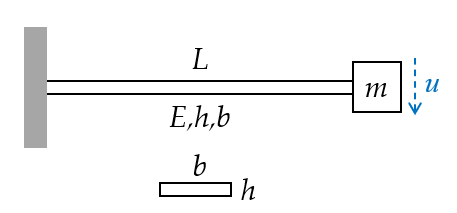
\includegraphics[width=0.72\linewidth,height=0.28\textheight,keepaspectratio]{figures/extracted-037.png}
\end{center}
\subsection{C.6 CALCULATE CANTILEVER RESPONSE TO SUDDENLY APPLIED}
\subsubsection*{Weight}

\begin{center}\small\itshape Figure 16: cantilever beam with tip mass\end{center}

Take g=9.81 m/s2 as the generally accepted value of gravitational acceleration. Consider a cantilever beam of length L=568 mm and a mass m=5.35kg that has to be attached to its tip as shown in Figure 16. The beam is made of steel with elastic modulus E=200 GPa and yield stress Y=710MPa cross-section properties h=3 mm, b=37 mm. Do the following:\par
\hangindent=2em\noindent\textbf{(1)} Display input data\par
\hangindent=2em\noindent\textbf{(2)} Calculate the cross-section second moment of area I, the flexural\par
stiffness EI, the spring constant k, the natural frequency ωn rad/s, fn Hz, and period of oscillation τ of the system\par
\hangindent=2em\noindent\textbf{(3)} Calculate the weight F0 of the mass m\par
\hangindent=2em\noindent\textbf{(4)} Static case: assume the mass is attached onto the undeformed\par
beam and the let go gradually without inducing any vibration and calculate the static displacement ust\par
\hangindent=2em\noindent\textbf{(5)} Dynamic case: assume the mass is attached onto the undeformed\par
beam and then let go suddenly inducing a state of vibration:\par
\hangindent=2em\noindent\textbf{(a)} calculate the maximum dynamic displacement udyn\par
\hangindent=2em\noindent\textbf{(b)} Plot the response u(t) measured from the undeformed\par
position for Nosc=10 oscillations\par
\hangindent=2em\noindent\textbf{(c)} Put a datatip on the plot to identify the maximum\par
displacement and compare with result of item (5)(a)\par
\hangindent=2em\noindent\textbf{(6)} Graduate work: calculate the maximum stress at the root of the\par
beam and the safety factor SF=Y/σ and comment on your results for the above two cases:\par
\hangindent=2em\noindent\textbf{(a)} σst for the static case\par
\hangindent=2em\noindent\textbf{(b)} σdyn for the dynamic case\par
\hangindent=2em\noindent\textbf{(7)} Discuss your results\par
\begin{center}
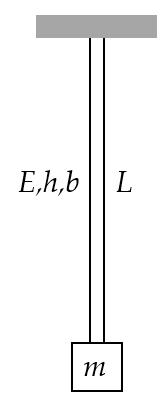
\includegraphics[width=0.72\linewidth,height=0.28\textheight,keepaspectratio]{figures/extracted-040.png}
\end{center}
\subsection{C.7 ANALYZE FLEX-BEAM PENDULUM}

\begin{center}\small\itshape Figure 17: flex-beam pendulum\end{center}

Consider a cantilever beam of length L with a mass m attached at its tip as shown in Figure 12. The beam is fixed into the ceiling and is hanging downward along the z axis. The mass may oscillate sideways in either x or y directions. The beam cross-section properties are E, h, b. Do the following:\par
\hangindent=2em\noindent\textbf{(1)} Calculate the minor and major second moments of area I1 and I2\par
\hangindent=2em\noindent\textbf{(2)} Assume a horizontal displacement u(t) which produces flexure\par
about the minor I1.\par
\hangindent=2em\noindent\textbf{(3)} Draw free-body diagram (FBD)\par
\hangindent=2em\noindent\textbf{(4)} Write Newton’s law of motion (NLM) equation\par
\hangindent=2em\noindent\textbf{(5)} Apply small-angle approximation and deduce the equation of\par
motion (EOM). Clearly state your assumptions.\par
\hangindent=2em\noindent\textbf{(6)} Define the natural frequency ωnFBP of the flex-beam pendulum\par
\hangindent=2em\noindent\textbf{(7)} Deduce the governing equation\par
\hangindent=2em\noindent\textbf{(8)} Compare your results with those of Problem B.1 and write the\par
general solution\par
\hangindent=2em\noindent\textbf{(9)} Solve the initial value problem (IVP), i.e., deduce the response\par
for simultaneous application of both initial displacement u0 and initial velocity u̇0\par
\hangindent=2em\noindent\textbf{(10)} Graduate Work: explain how the solution would change if\par
flexure was about I2\par
\begin{center}
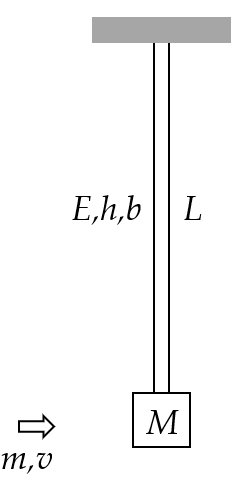
\includegraphics[width=0.72\linewidth,height=0.28\textheight,keepaspectratio]{figures/extracted-043.png}
\end{center}
\subsection{C.8 CALCULATE FLEX-BEAM PENDULUM RESPONSE TO IMPACT}

\begin{center}\small\itshape Figure 18: impact excitation of a vertical flex-beam pendulum\end{center}

Take g=9.81 m/s2 as the generally accepted value of gravitational acceleration. Consider a vertical flex-beam pendulum of length L=568 mm with a mass M=42 kg attached at its end as shown in\par
\begin{center}\small\itshape Figure 18. The beam material is steel with E=200 GPa. The beam\end{center}
cross-section dimensions are h=3 mm, b=37 mm. The beam is initially at rest. A projectile of mass m=18 grams and velocity v=935 m/s hits the mass and remains embedded into it. The azimuthal orientation of the projectile motion is such that the beam flexes about its minor cross-sectional stiffness. This impact imparts an initial velocity to the system that starts to oscillate. Do the following:\par
\hangindent=2em\noindent\textbf{(1)} Display input data\par
\hangindent=2em\noindent\textbf{(2)} Calculate the minor second moment of area I of the beam\par
\hangindent=2em\noindent\textbf{(3)} Calculate the minor cross-sectional stiffness EI\par
\hangindent=2em\noindent\textbf{(4)} Calculate the flex-beam spring constant k\par
\hangindent=2em\noindent\textbf{(5)} Calculate the initial velocity of the system u̇0 as resulting from\par
the interaction between the projectile and the large mass\par
\hangindent=2em\noindent\textbf{(6)} Calculate the rad/s natural frequency ωnFBP and period of\par
oscillation τFBP of the flex-beam pendulum with projectile embedded into it\par
\hangindent=2em\noindent\textbf{(7)} Calculate the response u(t1) after t1=10 sec\par
\hangindent=2em\noindent\textbf{(8)} Plot the response of the system for Nosc=10 oscillations and find\par
on the plot:\par
\hangindent=2em\noindent\textbf{(a)} the largest response\par
\hangindent=2em\noindent\textbf{(b)} the response value calculated at item (7)\par
\hangindent=2em\noindent\textbf{(9)} Discuss your results in comparison with results of Problem A.3\par
\subsection{C.9 COMPLEX EXPONENTIALS AND TRIGONOMETRIC}
\subsubsection*{Functions}

\hangindent=2em\noindent\textbf{(1)} Find the solutions of z4=1 (aka the fourth roots of unity) and\par
express them as\par
\hangindent=2em\noindent\textbf{(a)} complex numbers\par
\hangindent=2em\noindent\textbf{(b)} complex exponentials\par
\hangindent=2em\noindent\textbf{(2)} Write the complex number eiωt as a sum of trigonometric\par
functions (hint, Euler’s formula)\par
\hangindent=2em\noindent\textbf{(3)} Calculate the phase difference φ in radians and degrees between\par
the following signals\par
\hangindent=2em\noindent\textbf{(a)} x1(t)=sin(ωt), x2(t)=sin(ωt+3π/4)\par
\hangindent=2em\noindent\textbf{(b)} x1(t)=sin(ωt+π/3), x2(t)=sin(ωt+3π/4)\par
\hangindent=2em\noindent\textbf{(c)} x1(t)=sin(ωt+45o), x2(t)=sin(ωt+115o)\par
\hangindent=2em\noindent\textbf{(4)} What is the phase in radians and degrees of the following\par
complex numbers:\par
\hangindent=2em\noindent\textbf{(a)} eiπ/2\par
\hangindent=2em\noindent\textbf{(b)} ei3π/2\par
\hangindent=2em\noindent\textbf{(c)} eiπ/4\par
\hangindent=2em\noindent\textbf{(d)} e-iπ/2\par
\hangindent=2em\noindent\textbf{(e)} e-iπ/4\par
\hangindent=2em\noindent\textbf{(5)} Draw the locations on the unit circle of the complex numbers in\par
Section (3) above\par
\hangindent=2em\noindent\textbf{(6)} Calculate the magnitude and phase in degrees of the complex\par
number Z=4+5i\par
\end{document}
